\documentclass[orivec]{llncs}
\usepackage[utf8]{inputenc}
\usepackage{graphicx}
\usepackage{booktabs}
\usepackage[colorlinks=true, urlcolor=blue, linkcolor=blue]{hyperref}
\usepackage{xurl}
\usepackage{amsmath}

\title{Deep Learning Project: Chest X-ray Pneumonia Classification}
\author{Gorkem Baslik}
\institute{Università degli Studi di Milano Statale\\
\email{gorkem.baslik@studenti.unimi.it} \\ \vspace{0.2cm} March 19, 2026}

\begin{document}
\maketitle

\section{Dataset Version and Considered Data}
The dataset used in this project is sourced from Kaggle under the identifier \url{https://www.kaggle.com/datasets/yusufmurtaza01/chest-xray-pneumonia-balanced-dataset}. It contains chest X-ray images categorized into two classes: \textbf{NORMAL} and \textbf{PNEUMONIA}. The dataset was accessed on \textbf{March 14, 2026}. While the pipeline supports a ``quick mode'' subsampling technique to enforce strict runtime limits on constrained environments such as Google Colab, the experiments and results detailed in this report represent execution on the \textbf{full dataset} structure to demonstrate final predictive capability.

\section{Data Organization}
To stream the data dynamically during runtime, the project utilizes the official Kaggle API to download and extract the dataset, eliminating the need to track large file artifacts in the source repository. Once extracted, a custom indexing script recursively crawls the directory tree, mapping each valid image file (\texttt{.jpg}, \texttt{.jpeg}, \texttt{.png}, \texttt{.bmp}) to its respective label based on the parent folder name.

The complete corpus is subsequently divided using a \textbf{stratified split} into three partitions, strictly maintaining the class balance:
\begin{itemize}
  \item \textbf{Training Set:} 70\% of the data.
  \item \textbf{Validation Set:} 15\% of the data, used for hyperparameter tuning and early stopping.
  \item \textbf{Test Set:} 15\% of the data, isolated for final unbiased evaluation.
\end{itemize}
To ensure reproducibility, the precise file paths and labels for each split are recorded and exported permanently to \texttt{splits/train.csv}, \texttt{splits/val.csv}, and \texttt{splits/test.csv}.

\section{Pre-processing}
Prior to entering the neural network, raw images undergo a sequence of transformations mapping them to the expected input domain:
\begin{enumerate}
    \item \textbf{Resizing:} All images are uniformly resized to \(224 \times 224\) pixels to match the expected input resolution of the backbone network.
    \item \textbf{Data Augmentation (Training Only):} To combat overfitting and improve model generalization, multiple spatial and color jitter enhancements are randomly applied during training:
    \begin{itemize}
        \item Random Horizontal Flip ($p = 0.5$)
        \item Random Rotation (up to $\pm 10^\circ$)
        \item Color Jittering (Brightness: $\pm 0.1$, Contrast: $\pm 0.1$)
    \end{itemize}
    \item \textbf{Normalization:} After conversion to PyTorch tensors, inputs are standardized using the ImageNet pre-trained normalization parameters (mean: [0.485, 0.456, 0.406], std: [0.229, 0.224, 0.225]).
\end{enumerate}
Sanity visualization checks are included in the implementation pipeline to ensure artifacts apply meaningfully. 

\section{Algorithms and Implementation}
The core predictive algorithm leverages \textbf{Transfer Learning}. Specifically, we utilize a \textbf{Dense\-Net-121} architecture, pre-trained on ImageNet. This network effectively mitigates the vanishing-gradient problem and enforces feature propagation through dense block connections, thus establishing a strong baseline model for medical imaging tasks.

Implementation specifics include:
\begin{itemize}
    \item \textbf{Classifier Adaptation:} The original 1000-class fully connected layer is replaced by a simplified \texttt{nn.Linear(in\_features, 2)} structure outputting logits for the robust binary decision (NORMAL vs PNEUMONIA).
    \item \textbf{Fine-tuning Strategy:} By default, early features are frozen while parameters in deeper structural elements (e.g., \texttt{denseblock4} and \texttt{norm5}) can be unforced according to the hyperparameter search mechanism.
    \item \textbf{Optimization:} A standard \texttt{CrossEntropyLoss} coordinates penalization, actively minimized by the \texttt{AdamW} optimizer.
    \item \textbf{Early Stopping:} To prevent overfitting, validation F1 scores are continuously monitored. Optimization is halted if the metric fails to improve over 3 full epochs (patience = 3).
\end{itemize}
Performance tracking heavily prioritizes the \textbf{F1 Score} to holistically evaluate precision and recall balance, appended by tracking for Accuracy and ROC-AUC. 

\section{Scalability}
The programmatic pipeline is strictly designed to fulfill requirements on scalability:
\begin{itemize}
    \item \textbf{Quick Mode Switch:} A globally configurable \texttt{quick\_mode} parameter enforces strict limits on available samples (e.g., maximum 1200 train images, 250 validation, 250 test per class) per run. This allows rapid prototyping under the strict execution limits bound by Google Colab instances without code restructuring. 
    \item \textbf{Full Data Execution:} Switching \texttt{quick\_mode = False} directs the complete logic back equivalently against the full unconstrained dataset volume.
    \item \textbf{Computing Adjustments:} Configurable constants such as batch size (32 default) and worker counts implicitly scale load across distributed environments or standard multicore CPU deployments efficiently.
\end{itemize}

\section{Experiments}
Model selection was conducted under a constrained 4-trial budget navigating different critical hyperparameter setups. The search bounds assessed interactions between Learning Rate (\texttt{lr}), Weight Decay, Dropout regularizations, and the state of the final DenseNet feature blocks (Unfrozen vs Frozen).

Table 1 summarizes tuning performance natively recorded by the logging hooks. 

\begin{table}[htbp]
\centering
\caption{Hyperparameter Search Trials}
\renewcommand{\arraystretch}{1.2}
\setlength{\tabcolsep}{4pt}
\begin{tabular}{@{}cccccccc@{}}
\toprule
\textbf{Trial} & \textbf{Dropout} & \textbf{LR} & \textbf{Weight Decay} & \textbf{Unfreeze} & \textbf{Val F1} & \textbf{Epochs} & \textbf{Time (s)} \\ \midrule
1 & 0.2 & 1e-4 & 1e-4 & True  & \textbf{0.9835} & 8 & 1136 \\
2 & 0.3 & 3e-4 & 1e-5 & True  & 0.9820 & 8 & 1148 \\
3 & 0.4 & 1e-4 & 1e-5 & True  & 0.9773 & 5 & 775  \\
4 & 0.2 & 5e-4 & 1e-4 & False & 0.9354 & 8 & 1147 \\ \bottomrule
\end{tabular}
\end{table}

The optimal selection achieved a best \textbf{Validation F1 of \(\sim 0.9835\)}, emerging from unfreezing the final feature blocks and restricting to a \(1 \times 10^{-4}\) learning rate mapped alongside dropout 0.2.

\section{Results and Discussion}
Evaluating the definitive best model (from Trial 1) across the isolated 1280-image Test Split yields striking robustness:
\begin{itemize}
    \item \textbf{Accuracy:} 98.20\%
    \item \textbf{F1-score:} 98.20\%
    \item \textbf{Precision:} 98.58\%
    \item \textbf{Recall:} 97.81\%
    \item \textbf{ROC AUC:} 0.9974
\end{itemize}

\begin{figure}[htbp]
    \centering
    % Note: Save your Confusion Matrix & ROC plot from main.ipynb as 'reports/cm_roc.png'
    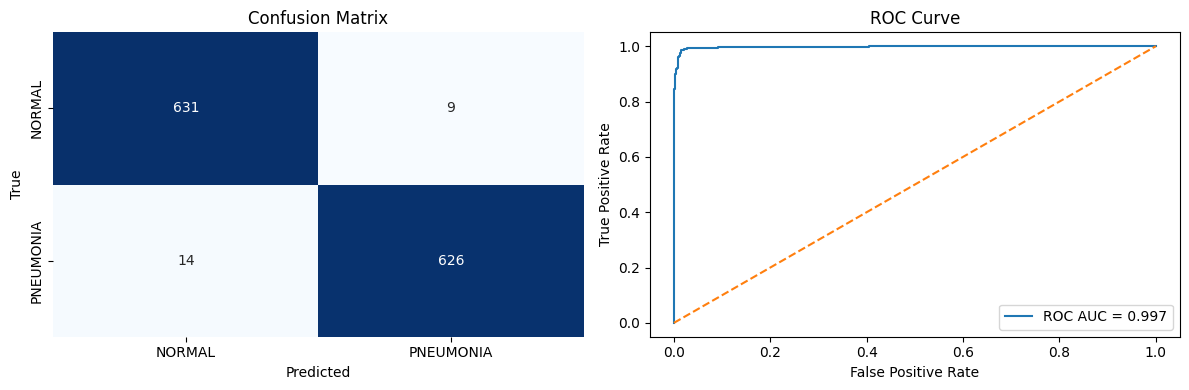
\includegraphics[width=1\textwidth]{reports/cm_roc.png}
    \caption{Confusion Matrix and ROC Curve summarizing test set evaluation performance.}
    \label{fig:cm_roc}
\end{figure}

The highly symmetric classification profile validates effective abstraction and minimal class bias. As indicated continuously over the detailed classification report, predicting both Normal and Pneumonia subsets yielded analogous performance characteristics (Normal Recall: 99\%, Pneumonia Recall: 98\%). 

\textbf{Explainability (Grad-CAM):}
To trace network behavior, \textbf{Grad-CAM visualization} was utilized, intersecting output feature activations overlapping original X-Ray films (see Figure \ref{fig:gradcam}). True Positive cases demonstrate correct activation localization toward lungs revealing symptomatic consolidations. False Positives instances occasionally hallucinate non-specific artifacts (e.g., skeletal structures overlapping lung periphery) mimicking ground-glass opacity behavior typical of pneumonia.

\begin{figure}[htbp]
    \centering
    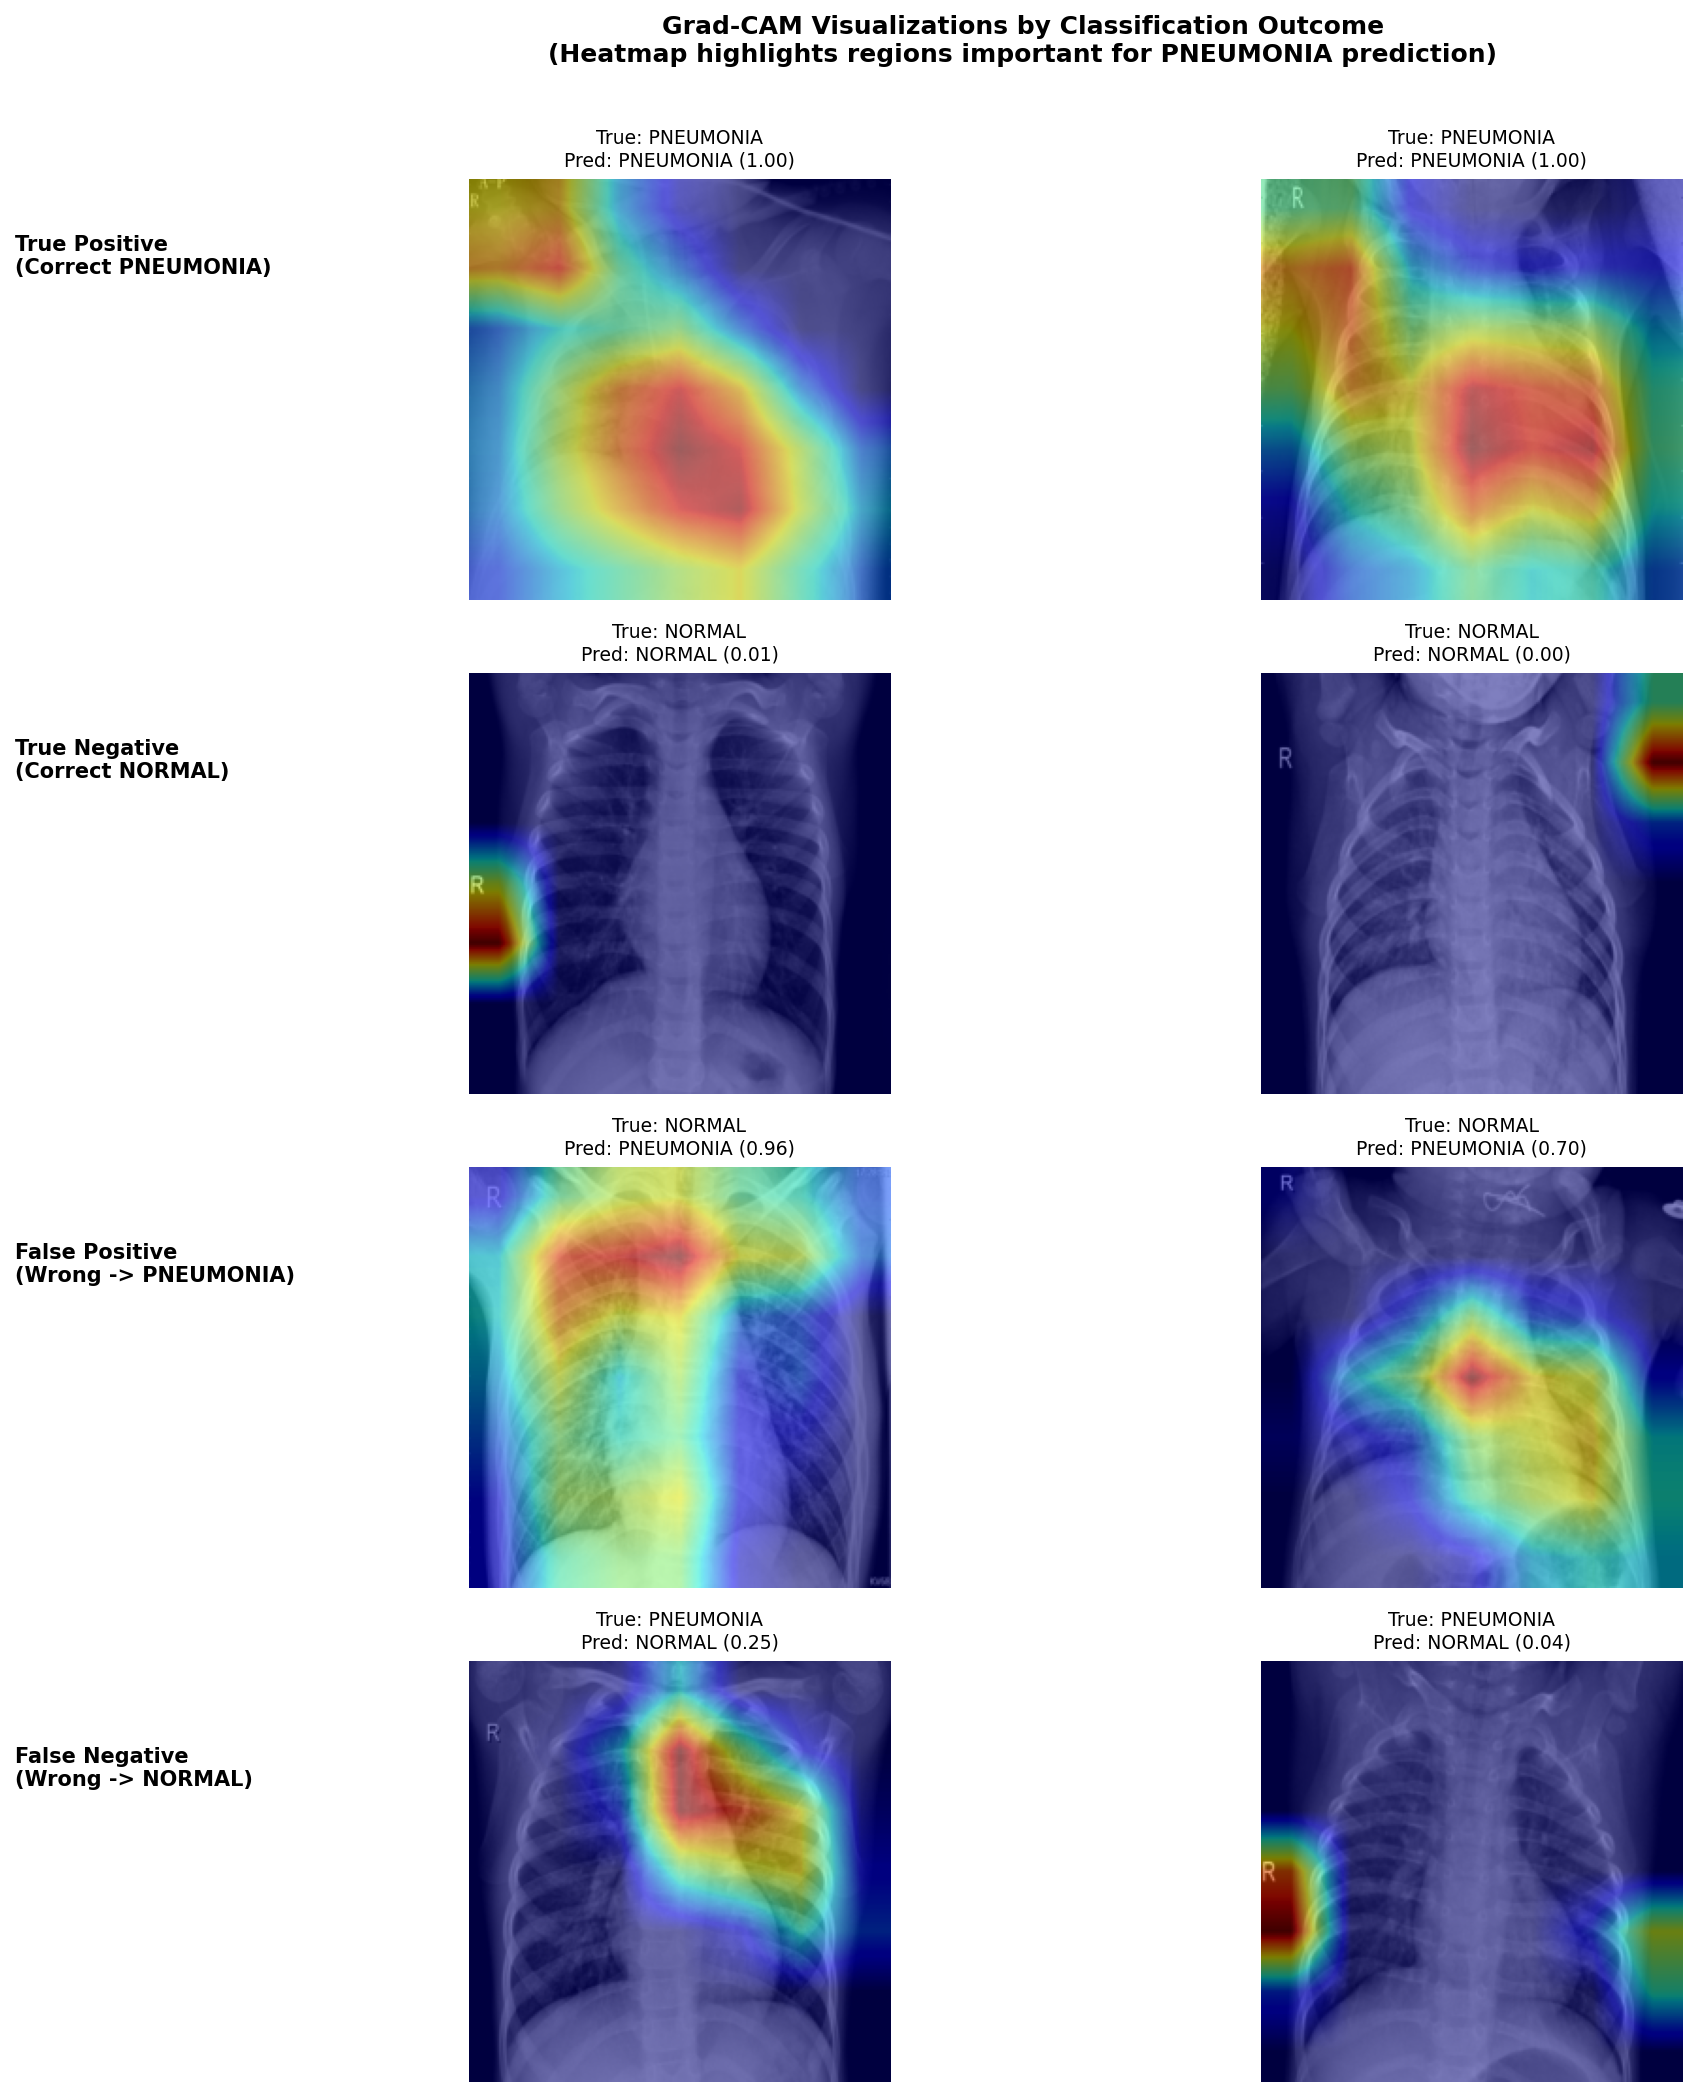
\includegraphics[width=1\textwidth]{reports/gradcam_analysis.png}
    \caption{Grad-CAM Visualizations for True/False Positives and Negatives highlighting important regions for prediction.}
    \label{fig:gradcam}
\end{figure}

\section{Reproducibility Notes}
To guarantee repeatable results, follow these critical measures:
\begin{itemize}
    \item Full code is available on GitHub: \url{https://github.com/gorkembaslik/deep-learning}
    \item Set \texttt{Config.seed = 42}.
    \item Due to constraints around public repositories, actual Kaggle API keys reside as \texttt{xxxxxx} string placeholders in the root submission block. User credentials must be replaced manually before rerunning Google Colab cells.
    \item Ensure \texttt{quick\_mode = False} dictates global behavior to duplicate the full data distribution.
\end{itemize}
\newpage
I/We declare that this material, which I/We now submit for assessment, is entirely my/our own work and has not been taken from the work of others, save and to the extent that such work has been cited and acknowledged within the text of my/our work. I/We understand that plagiarism, collusion, and copying are grave and serious offences in the university and accept the penalties that would be imposed should I engage in plagiarism, collusion or copying. This assignment, or any part of it, has not been previously submitted by me/us or any other person for assessment on this or any other course of study. No generative AI tool has been used to write the code or the report content.
\end{document}
